\section[PKI and blockchains]{Background on public key infrastructure (PKI) and blockchains}

\begin{frame}{Public key infrastructure}
A \mg{public key infrastructure (PKI)} is a set of roles, policies, and procedures needed to create, manage, distribute, use, store, and revoke digital certificates and manage public-key encryption.

\vspace{2mm}

PKI involves
\begin{itemize}
\item public key cryptography,
\item digital certificates,
\item digital identity management.
\end{itemize}

\end{frame}


\begin{frame}{Public key infrastructure}
\begin{figure}[t]
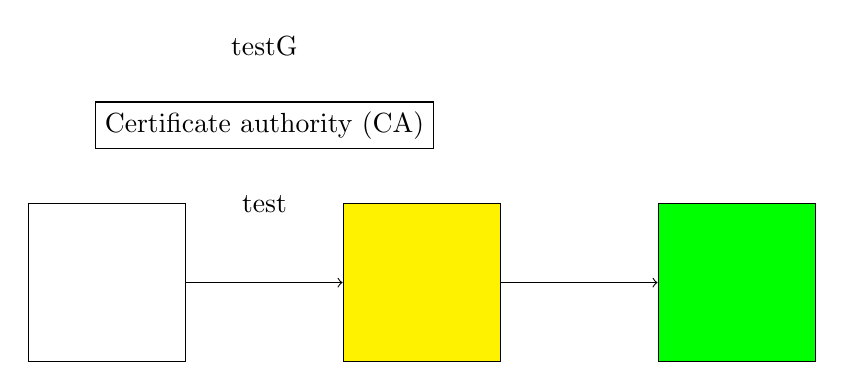
\begin{tikzpicture}
\node[draw,rectangle,
inner xsep=1cm,inner ysep=1cm,
fill=white](user) at (-30,0){};

\node[] (lab) at (-28, 1){test};

\node[] (laba) at (-28, 3){testG};

%\node[draw,circle,
%inner xsep=0.2cm,inner ysep=0.2cm,
%fill=white](ca) at (-28,2){Certificate authority (CA)};

\node[draw,rectangle,
fill=white](ca) at (-28,2){Certificate authority (CA)};

\node[draw,rectangle,
inner xsep=1cm,inner ysep=1cm,
fill=yellow](cert) at (-26,0){};

\node[draw,rectangle,
inner xsep=1cm,inner ysep=1cm,
fill=green](repo) at (-22,0){};


\draw [->] (user) to (cert);
\draw [->] (cert) to (repo);
\end{tikzpicture}
\end{figure}

a figure to be placed here, based on IDNOMIC's page 6
\end{frame}


\begin{frame}
\begin{figure}[ht]
\center
\begin{tikzpicture}
\node[circle,inner xsep=3cm,inner ysep=0cm,draw](C){};  
% the circle is a node, that way I can tell it to put other nodes at its north, east, west, etc
% inner xsep and inner ysep are for the rectangle that fits inside the circle
% because for some obscure reason this is how tikz works
% anyways this is how you get a circle with a 5cm radius :)
%\node[draw,fill,circle,inner sep=4pt,label=above left:{1}](O) at (C.center){};

\node[] (O) at (C.center){};	%to refer to the center of C by O
 
% I drew a small circular black dot at the center of the circle C and called it O, 
% inner sep is for the length between the center and the exterior of the node
% and the label is in the [] because it's not /in/ the node but "above left" :)


\node[draw,circle,label=left:{$x_1$},fill=white](xi) at (C.west){};
\node[draw,circle,label=right:{$x_2$},fill=white](xj) at (C.east){};

\node[draw,circle,label=left:{$x_1^+$},pattern=lines](xi+) at ($(O)+(160:3cm)$){};
\node[draw,circle,label=left:{$x_1^-$},fill=white](xi-) at ($(O)+(200:3cm)$){};
\node[draw,circle,label=above left:{$y_1^-$},pattern=lines](yi-) at ($(O)+(120:3cm)$){};
\node[draw,circle,label=above left:{$y_1$},pattern=lines](yi) at ($(O)+(100:3cm)$){};

\node[draw,circle,label=above:{$u_1$},fill=white](u1) at ($(O)-(0:2cm)$){}; 
\node[draw,circle,label=above:{$u_r$},fill=white](ur) at ($(O)+(0:2cm)$){}; 

\node[draw,circle,label=right:{$x_2^-$},fill=white](xj-) at ($(O)+(20:3cm)$){};
\node[draw,circle,label=right:{$x_2^+$},pattern=cross](xj+) at ($(O)+(340:3cm)$){};
\node[draw,circle,label=below right:{$y_2^-$},pattern=cross](yj-) at ($(O)+(300:3cm)$){};
\node[draw,circle,label=below right:{$y_2$},pattern=cross](yj) at ($(O)+(280:3cm)$){};

% this one is placed according to an angle, 40, at 5cm from the center O, i.e., on the line of C :)
\draw (xi) to (u1);
\draw (u1) to (ur);
\draw (ur) to (xj);
\draw (xi) to (yi-);
\draw[dashed] (xi) to (yi);
\draw (xj) to (yj-);
\draw[dashed] (xj) to (yj);
\draw[-,bend left] (xi-) to (xi+);	%perhaps improve
% this is a solid line from n2 to O :)
\end{tikzpicture}
\caption{The subgraph $C\cup P$ of $G$. Vertices $z_1$ are marked with
horizontal stripes and vertices $z_2$ with crossing lines.}
\end{figure}
\end{frame}


\begin{frame}{Public key infrastructure}

certificates, chain of trust

\end{frame}

\begin{frame}{Blockchain definition}

\begin{itemize}
\item A \mg{blockchain} is a public, transparent,
append-only ledger
%\pause
\item Created by members of a peer-to-peer
network
\item bzzzzz
\item kleklekle
\end{itemize}

definition
\end{frame}



\begin{frame}{Blockchain structure}

\begin{itemize}
\item A \mg{blockchain} is a public, transparent,
append-only ledger
%\pause
\item Created by members of a peer-to-peer
network
\item bzzzzz
\item kleklekle
\end{itemize}

\end{frame}
